%!TEX root = ../Studienarbeit.tex

\chapter{Einleitung}

Multikopter beziehungsweise Quadrokopter haben in den letzten Jahren sowohl im privaten als auch im kommerziellen Sektor ein konstantes Wachstum hingelegt. So sind beispielsweise in den Vereinigten Staaten von Amerika zum Stand vom 31. Mai 2022 über 865.000 Multikopter registriert. Davon sind über 500.000 Multikopter privat und über 300.000 für die kommerzielle Nutzung registriert. \cites{droneregistrationFAA}{dronestat1}{dronestat2}{dronestat3}

Quadrokopter lassen sich grob in zwei Kategorien einteilen. Zum einen die Consumerquadrokopter, welche viele  Sensoren enthalten, um Unterstützungsfunktionen den teils ungeübten Piloten bereitzustellen. Ein Beispiel für einen Quadrokopter dieser Kategorie wäre die Mavic 3 Classic von dem Unternehmen DJI. Diese hat beispielsweise Sichtsensoren welche nach unten, oben, vorne und hinten ausgerichtet sind, um Objekte im Flugfeld auszuweichen. Ebenso unterstützt dieser Quadrokopter den automatischen Rückflug an den Startpunkt. Eine weitere Hilfsfunktion, welche in diesem Quadrokopter implementiert ist, ist die Möglichkeit beide Steuerknüppel loszulassen wobei der Quadrokopter stabil die Lage in der Luft hält. \cite{djiMavicClassic}

Die zweite Kategorie von Quadrokoptern sind sogenannte Freestyle- beziehungsweise Rennquadrokopter. Diese sind im Gegensatz zu den Consumerquadrokoptern dazu ausgelegt möglichst leicht zu sein, um möglichst schnelle und beeindruckende Manöver machen zu können. Dafür wird jedoch auf die Unterstützungsfunktionen von Consumerquadrokoptern verzichtet. Eine weitere Besonderheit ist die Möglichkeit zwischen drei Flugmodi auszuwählen. Zum einen den Flugmodus \textit{Angle Mode} dabei wird der Quadrokopter ab einen fest vordefinierten Neigungswinkel automatisch begrenzt, wodurch Loopings und Rollen des Quadrokopters unterbunden werden. Ebenso dreht sich der Quadrokopter wieder in die Ausgangslage zurück, wenn die Steuerknüppel zentriert werden. Der zweite Flugmodus ist der \textit{Horizon Mode}, dieser bietet wie der \textit{Angle Mode} die Funktion, dass sich der Quadrokopter wieder zur Ausgangslage zurückdreht, wenn die Steuerknüppel in die zentrale Stellung zurückgebracht werden. Jedoch können in diesen Flugmodus Loopings und Rollen gemacht werden. Der letzte verfügbar Flugmodus ist der \textit{Air beziehungsweise Acro Mode}. In diesen Modus muss der Pilot sich um das Ausrichten der Drohne in alle Drehrichtungen kümmern, da bei Loslassen der Steuerknüppel die vorhanden Drehungen des Quadrokopters beibehalten werden. Dieser Modus wird von Freestyle und Rennpiloten meist verwendet. In Abbildung \ref{fig:flugmodi} ist eine Übersicht aller Flugmodi zu sehen. \cite{wedioFlugmodi}

\begin{figure}[h]
    \centering
    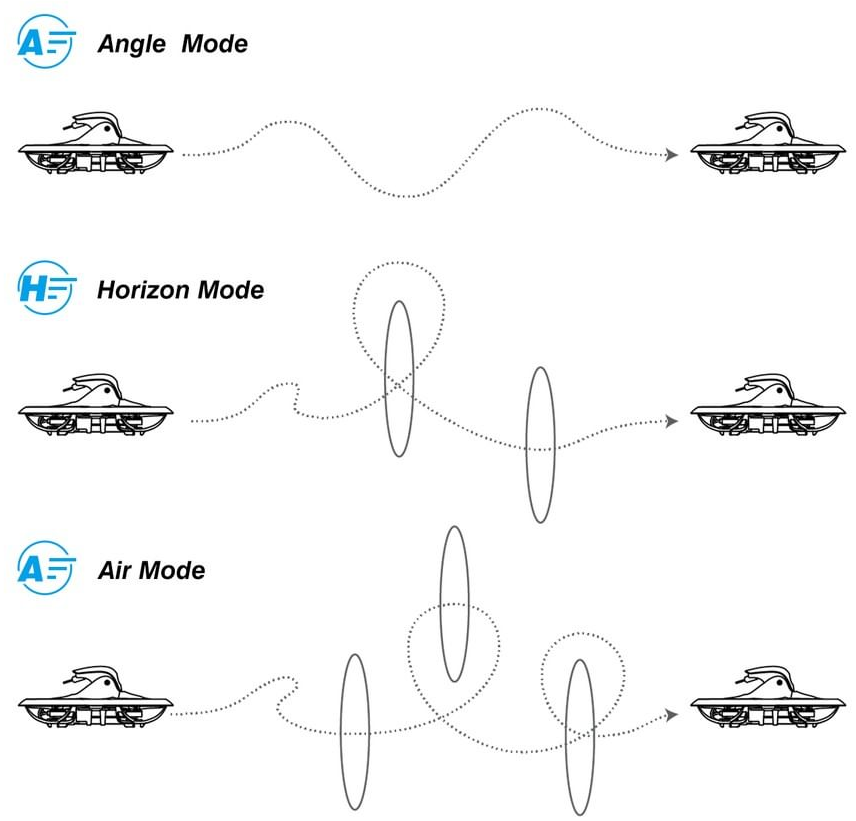
\includegraphics[width=.25\paperheight]{flugmodi}
    \caption{Verfügbaren Flugmodi bei Freestyle beziehungsweise Rennquadrokoptern; angepasst von \cite{betafpvFlugmodi}}
    \label{fig:flugmodi}
\end{figure}

Neben dem Multikopterfliegen stellt für Renn- und Freestyle-Quadrokopterpiloten das Training ein wichtiger Bestandteil dar, um die Bedienung des Quadrokopters im \textit{Air beziehungsweise Acro Mode} zu verbessern. Das Training kann in zwei Varianten durchgeführt werden. Der Quadrokopterpilot trainiert entweder am Flugplatz. Hier können aber durch Abstürze hohe Reparaturkosten und lange Reparaturzeiten entstehen. Oder der Quadrokopterpilot trainiert im Simulator am Rechner, wodurch keine Reparaturkosten und Reparaturzeiten entstehen.

\section{Motivation}

Da in den letzten Jahren das Unternehmen Apple Tablets mit leistungsstarken Prozessoren, welche ursprünglich für Notebooks und Desktops gedacht waren, entwickelt hat \cite{appleM2IPad}, wäre es wünschenswert Quadrokopter-Simulatoren für die immer leistungsfähigeren mobilen Geräte bereitzustellen. Hierfür muss jedoch die Möglichkeit bestehen die gewohnte Fernsteuerung der Quadrokopter mit Endgeräten zu verbinden, um den Piloten eine gewohnte Umgebung zu bieten. Die Verbindung einer Fernsteuerung mit einem Endgerät bieten einige Hersteller an, indem sich die Fernsteuerung per USB als USB-\acs{HID}-Joystick identifiziert \cite{opentxJoystick}. Das Problem hierbei ist jedoch, dass die Verbindung mittels USB mit mobilen Geräten nur eingeschränkt beziehungsweise unmöglich ist herzustellen. Beseitigt werden kann dieses Problem bei Fernsteuerung mit Modulschächten \cite{opentxModulbay}, mit deren Hilfe  die Tasten- und Joysticksignale über andere Funkstandard übertragen werden können.

Ziel der Arbeit ist es daher ein Hardware-Erweiterungsmodul für Multikopterfernsteuerungen zu entwickeln, womit eine Fernsteuerung mit einem Endgerät verbunden werden kann, welches nicht USB zu Datenübertragung bereitstellen.

\section{Stand der Technik}

Damit Fernsteuerungen von Quadrokoptern an Computern für das Training am Simulator verwendet werden können, gibt es zurzeit drei Möglichkeiten. Die erste Möglichkeit ist es die Fernsteuerung von ausgewählten Herstellern mittels USB zu verbinden. Dadurch wird die Fernsteuerung am Computer als USB-\acs{HID}-Joystick erkannt \cite{opentxJoystick}. Die zweite Möglichkeit ist es, den Quadrokopter auf dem die Firmware Betaflight vorhanden ist mittels USB anzustecken und diesen als Empfänger für die Fernsteuerung zu verwenden \cite{betaflightHID}. Da diese zwei Möglichkeiten jeweils USB zur Datenübertragung verwenden, sind diese Varianten nicht für alle Endgeräte geeignet. Die letzte Möglichkeit ist es an Fernsteuerung mit Erweiterungsmodulschacht ein Hardwaremodul zu verwenden, welche die Daten mittels Bluetooth übertragen. Hierbei ist als einziges bekanntes Modul das Modul des Unternehmens Orqa zu nennen \cite{orqaBluetoothModule}. Dieses Modul ist jedoch nur für Modulschächte des Typs JR geeignet und nicht für Modulschächte des Typs Lite.